\documentclass{standalone}
\usepackage{tikz}
\usepackage{ctex}
\setCJKmainfont{Noto Serif CJK SC}
\usepackage{mhchem,siunitx}
\begin{document}
\large
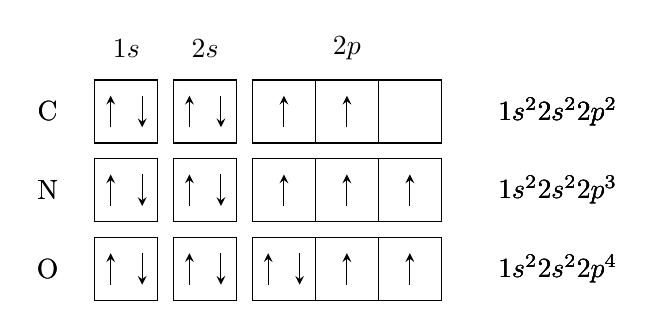
\begin{tikzpicture}[scale=1.0,>=stealth]
  \foreach \x in {0,1}
    {
      \foreach \y/\s in {0/C,-1/N,-2/O}
      {
        \draw(\x,\y)rectangle++(0.8,0.8);
        \draw[->](\x+0.2,\y+0.2)--++(0,0.4);
        \draw[->](\x+0.6,\y+0.6)--++(0,-0.4);
        \node at (-0.6,\y+0.4) {\ce{\s}};
      }
    }
  \foreach \x in {2,2.8,3.6}
    {
      \foreach \y/\s in {0/1s^22s^22p^2,-1/1s^22s^22p^3,-2/1s^22s^22p^4}
        {
          \draw(\x,\y)rectangle++(0.8,0.8);
          \node at (5,\y+0.4)[right]{$\s$};
        }
    }
  \draw[->](2.4,0.2)--++(0,0.4);
  \draw[->](3.2,0.2)--++(0,0.4);
  \draw[->](2.4,-0.8)--++(0,0.4);
  \draw[->](3.2,-0.8)--++(0,0.4);
  \draw[->](4.0,-0.8)--++(0,0.4);
  \draw[->](2.2,-1.8)--++(0,0.4);
  \draw[->](2.6,-1.4)--++(0,-0.4);
  \draw[->](3.2,-1.8)--++(0,0.4);
  \draw[->](4.0,-1.8)--++(0,0.4);
  
  \foreach \x/\y in {0.4/1s,1.4/2s,3.2/2p}
  {
    \node at (\x,1.2) {$\y$};
  }
  \node at (5,0.4)[right]{$1s^22s^22p^2$};
\end{tikzpicture}
\end{document}